\documentclass[12pt,a4paper]{report}
\usepackage[utf-8]{inputenc}
\usepackage[margin=1in]{geometry}
\usepackage{graphicx}
\usepackage{subcaption}
\usepackage{float}
\usepackage{hyperref}
\usepackage{amsmath}
\usepackage{amssymb}
\usepackage{booktabs}
\usepackage{array}
\usepackage{xcolor}
\usepackage{fancyhdr}
\usepackage{lastpage}
\usepackage{tabularx}
\usepackage{listings}
\usepackage{color}

% Define colors for listings
\definecolor{codegreen}{rgb}{0,0.6,0}
\definecolor{codegray}{rgb}{0.5,0.5,0.5}
\definecolor{codepurple}{rgb}{0.58,0,0.82}
\definecolor{backcolour}{rgb}{0.95,0.95,0.92}

\lstdefinestyle{mystyle}{
    backgroundcolor=\color{backcolour},
    commentstyle=\color{codegreen},
    keywordstyle=\color{codepurple},
    numberstyle=\tiny\color{codegray},
    stringstyle=\color{codepurple},
    basicstyle=\ttfamily\footnotesize,
    breakatwhitespace=false,
    breaklines=true,
    captionpos=b,
    keepspaces=true,
    numbers=left,
    numbersep=5pt,
    showspaces=false,
    showstringspaces=false,
    showtabs=false,
    tabsize=2
}

\lstset{style=mystyle}

% Header and footer
\pagestyle{fancy}
\fancyhf{}
\fancyhead[L]{DINDGA Project Report}
\fancyhead[R]{\thepage\ of \pageref{LastPage}}
\fancyfoot[C]{Generated: \today}

\title{
    \textbf{Dynamic Network Intrusion Detection\\
    Graph Analyzer (DINDGA)}\\
    \large{Final Project Report}
}
\author{
    Your Name\\
    University/Institution\\
    \date{\today}
}

\date{\today}

\begin{document}

\maketitle

\tableofcontents
\newpage

% ============================================================================
% CHAPTER 1: INTRODUCTION
% ============================================================================
\chapter{Introduction}

\section{Project Overview}

The Dynamic Network Intrusion Detection Graph Analyzer (DINDGA) is a comprehensive system designed to detect and analyze network intrusions using graph-based analysis techniques. This report presents the analysis results, visualizations, and findings from the implementation.

\section{Objectives}

\begin{itemize}
    \item Analyze network traffic data to identify anomalous behavior
    \item Build a dynamic graph representation of network connections
    \item Detect potential intrusions and security threats
    \item Generate comprehensive visualizations for security analysis
    \item Provide actionable insights for network administrators
\end{itemize}

\section{Dataset Description}

The analysis is based on network traffic data collected from [INSERT NETWORK DESCRIPTION]. The dataset includes:

\begin{itemize}
    \item Network traffic flows with protocols, IP addresses, and ports
    \item Packet and byte count information
    \item Temporal information (duration of connections)
    \item Traffic labels (Normal vs Attack)
    \item Threat detection results and anomaly scores
\end{itemize}

% ============================================================================
% CHAPTER 2: METHODOLOGY
% ============================================================================
\chapter{Methodology and Implementation}

\section{System Architecture}

The DINDGA system consists of the following main components:

\begin{enumerate}
    \item \textbf{Data Processing Module}: Loads and preprocesses network data
    \item \textbf{Graph Building Component}: Constructs dynamic network graphs
    \item \textbf{Intrusion Detection Engine}: Applies detection algorithms
    \item \textbf{Visualization Module}: Generates analytical plots and reports
\end{enumerate}

\section{Detection Algorithms}

\subsection{Anomaly Detection}

The system uses multiple approaches to detect anomalies:

\begin{itemize}
    \item \textbf{Isolation Forest}: Identifies anomalous patterns in high-dimensional data
    \item \textbf{Temporal Analysis}: Detects connection spikes and temporal patterns
    \item \textbf{Graph Metrics}: Analyzes node degree, clustering coefficients, and centrality
\end{itemize}

\subsection{Threat Scoring}

Threat scores are calculated using a combination of factors:
\begin{equation}
\text{ThreatScore} = w_1 \cdot \text{Anomaly} + w_2 \cdot \text{Degree} + w_3 \cdot \text{PortDiversity} + w_4 \cdot \text{Temporal}
\end{equation}

Where $w_i$ are weights determined through analysis and validation.

\section{Implementation Details}

The system is implemented in Python using the following key libraries:

\begin{itemize}
    \item \textbf{pandas}: Data manipulation and analysis
    \item \textbf{NetworkX}: Graph construction and analysis
    \item \textbf{scikit-learn}: Machine learning algorithms
    \item \textbf{matplotlib/seaborn}: Visualization
    \item \textbf{Streamlit}: Interactive web interface
\end{itemize}

% ============================================================================
% CHAPTER 3: RESULTS AND ANALYSIS
% ============================================================================
\chapter{Results and Analysis}

\section{Data Overview}

\begin{table}[H]
\centering
\caption{Summary Statistics}
\begin{tabularx}{\textwidth}{|l|X|X|}
\hline
\textbf{Metric} & \textbf{Category} & \textbf{Value} \\
\hline
Total Records & Network Data & [INSERT VALUE] \\
\hline
Unique Source IPs & Network Data & [INSERT VALUE] \\
\hline
Unique Destination IPs & Network Data & [INSERT VALUE] \\
\hline
Total IPs Analyzed & Detection Results & [INSERT VALUE] \\
\hline
High Threat IPs & Detection Results & [INSERT VALUE] \\
\hline
Total Alerts & Threat Alerts & [INSERT VALUE] \\
\hline
\end{tabularx}
\end{table}

Import the summary statistics from \texttt{summary\_statistics.csv} for the actual values.

\section{Traffic Classification}

\subsection{Label Distribution}

\begin{figure}[H]
\centering
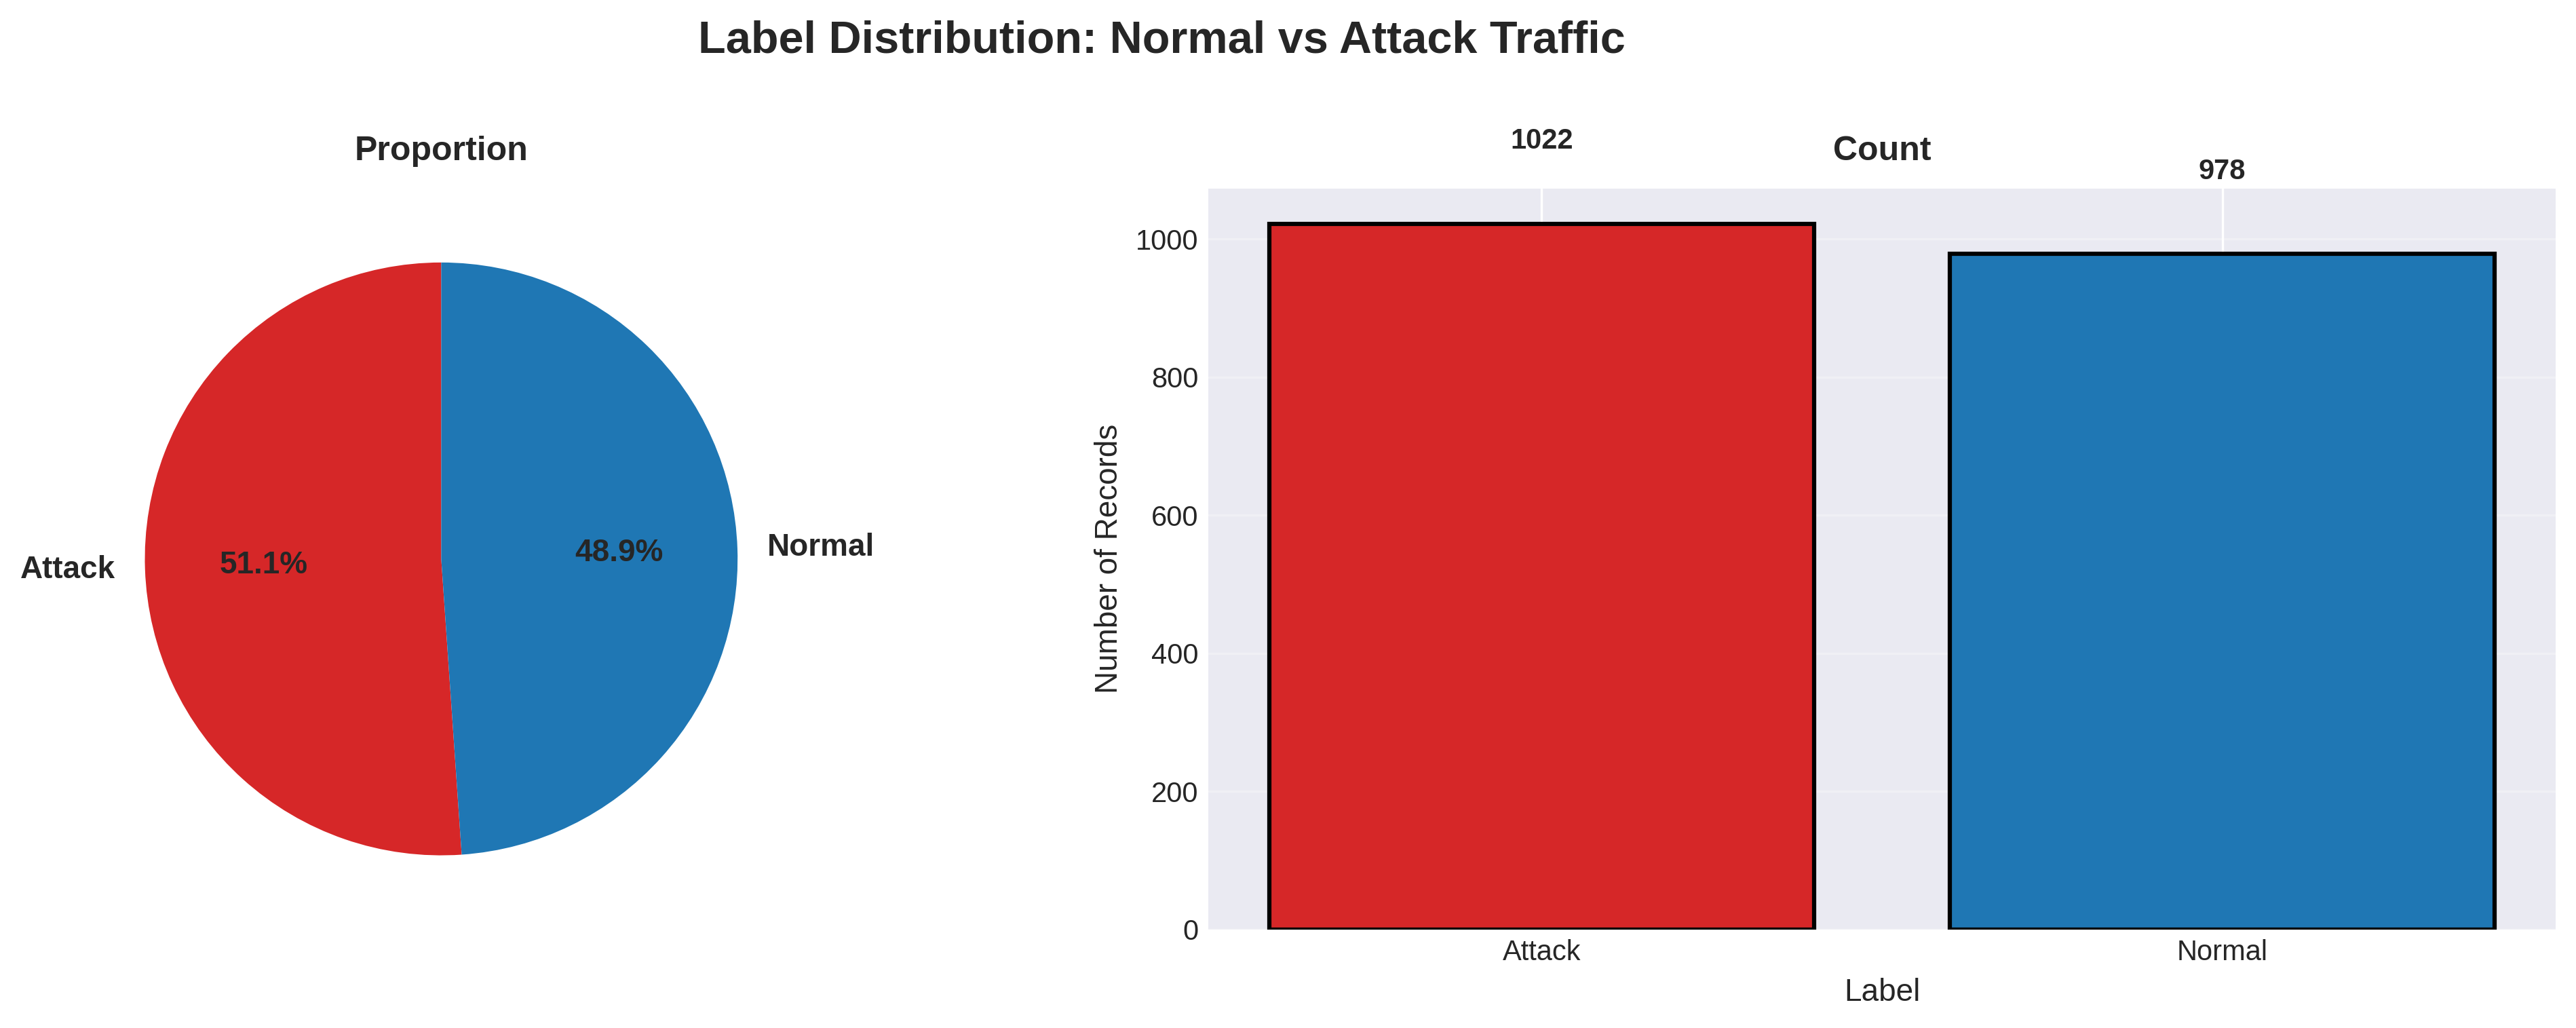
\includegraphics[width=0.9\textwidth]{plots/01_label_distribution.png}
\caption{Distribution of Normal and Attack Traffic. The pie chart shows the proportion of traffic labels, while the bar chart displays absolute counts.}
\label{fig:label_dist}
\end{figure}

Key observations:
\begin{itemize}
    \item [INSERT OBSERVATIONS ABOUT TRAFFIC CLASSIFICATION]
    \item Proportions indicate the balance between normal and attack traffic
    \item This distribution can be used to understand the attack prevalence in the dataset
\end{itemize}

\section{Network Topology Analysis}

\subsection{IP Degree Distribution}

\begin{figure}[H]
\centering
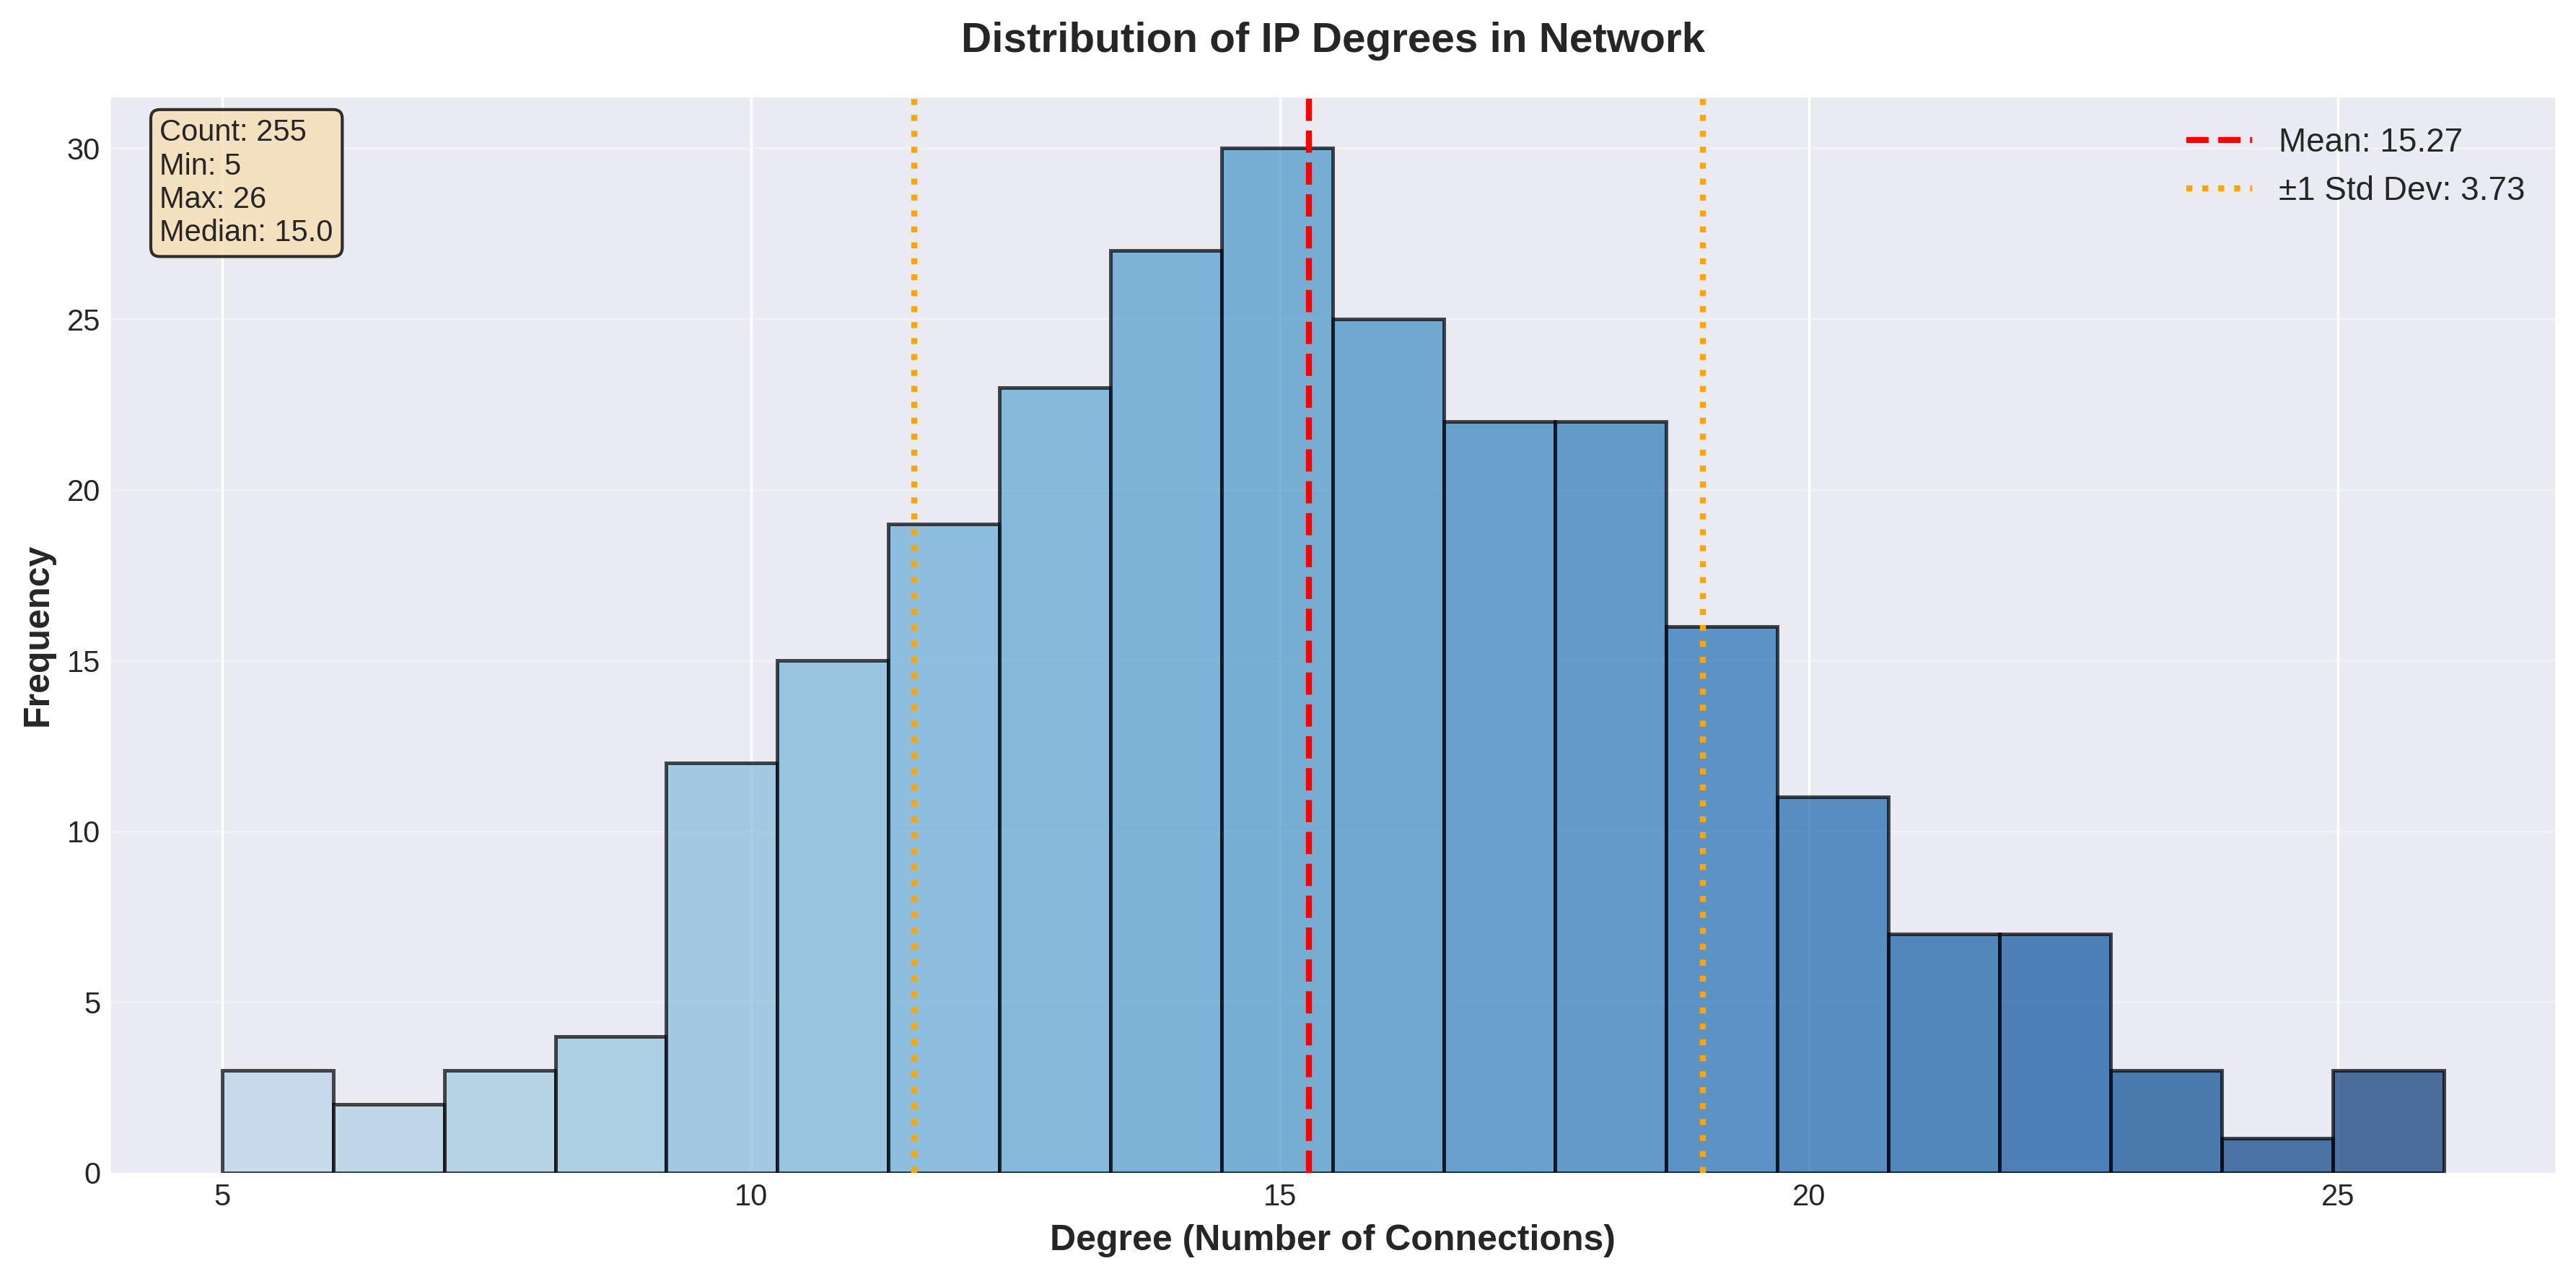
\includegraphics[width=0.9\textwidth]{plots/02_degree_distribution.png}
\caption{Histogram showing the distribution of IP node degrees in the network graph. The degree represents the number of unique connections for each IP address.}
\label{fig:degree_dist}
\end{figure}

Analysis:
\begin{itemize}
    \item The degree distribution provides insight into network connectivity patterns
    \item IPs with unusually high or low degrees may indicate suspicious behavior
    \item The mean and standard deviation help identify outliers
\end{itemize}

\section{Threat Detection Results}

\subsection{Top Threat IPs}

\begin{figure}[H]
\centering
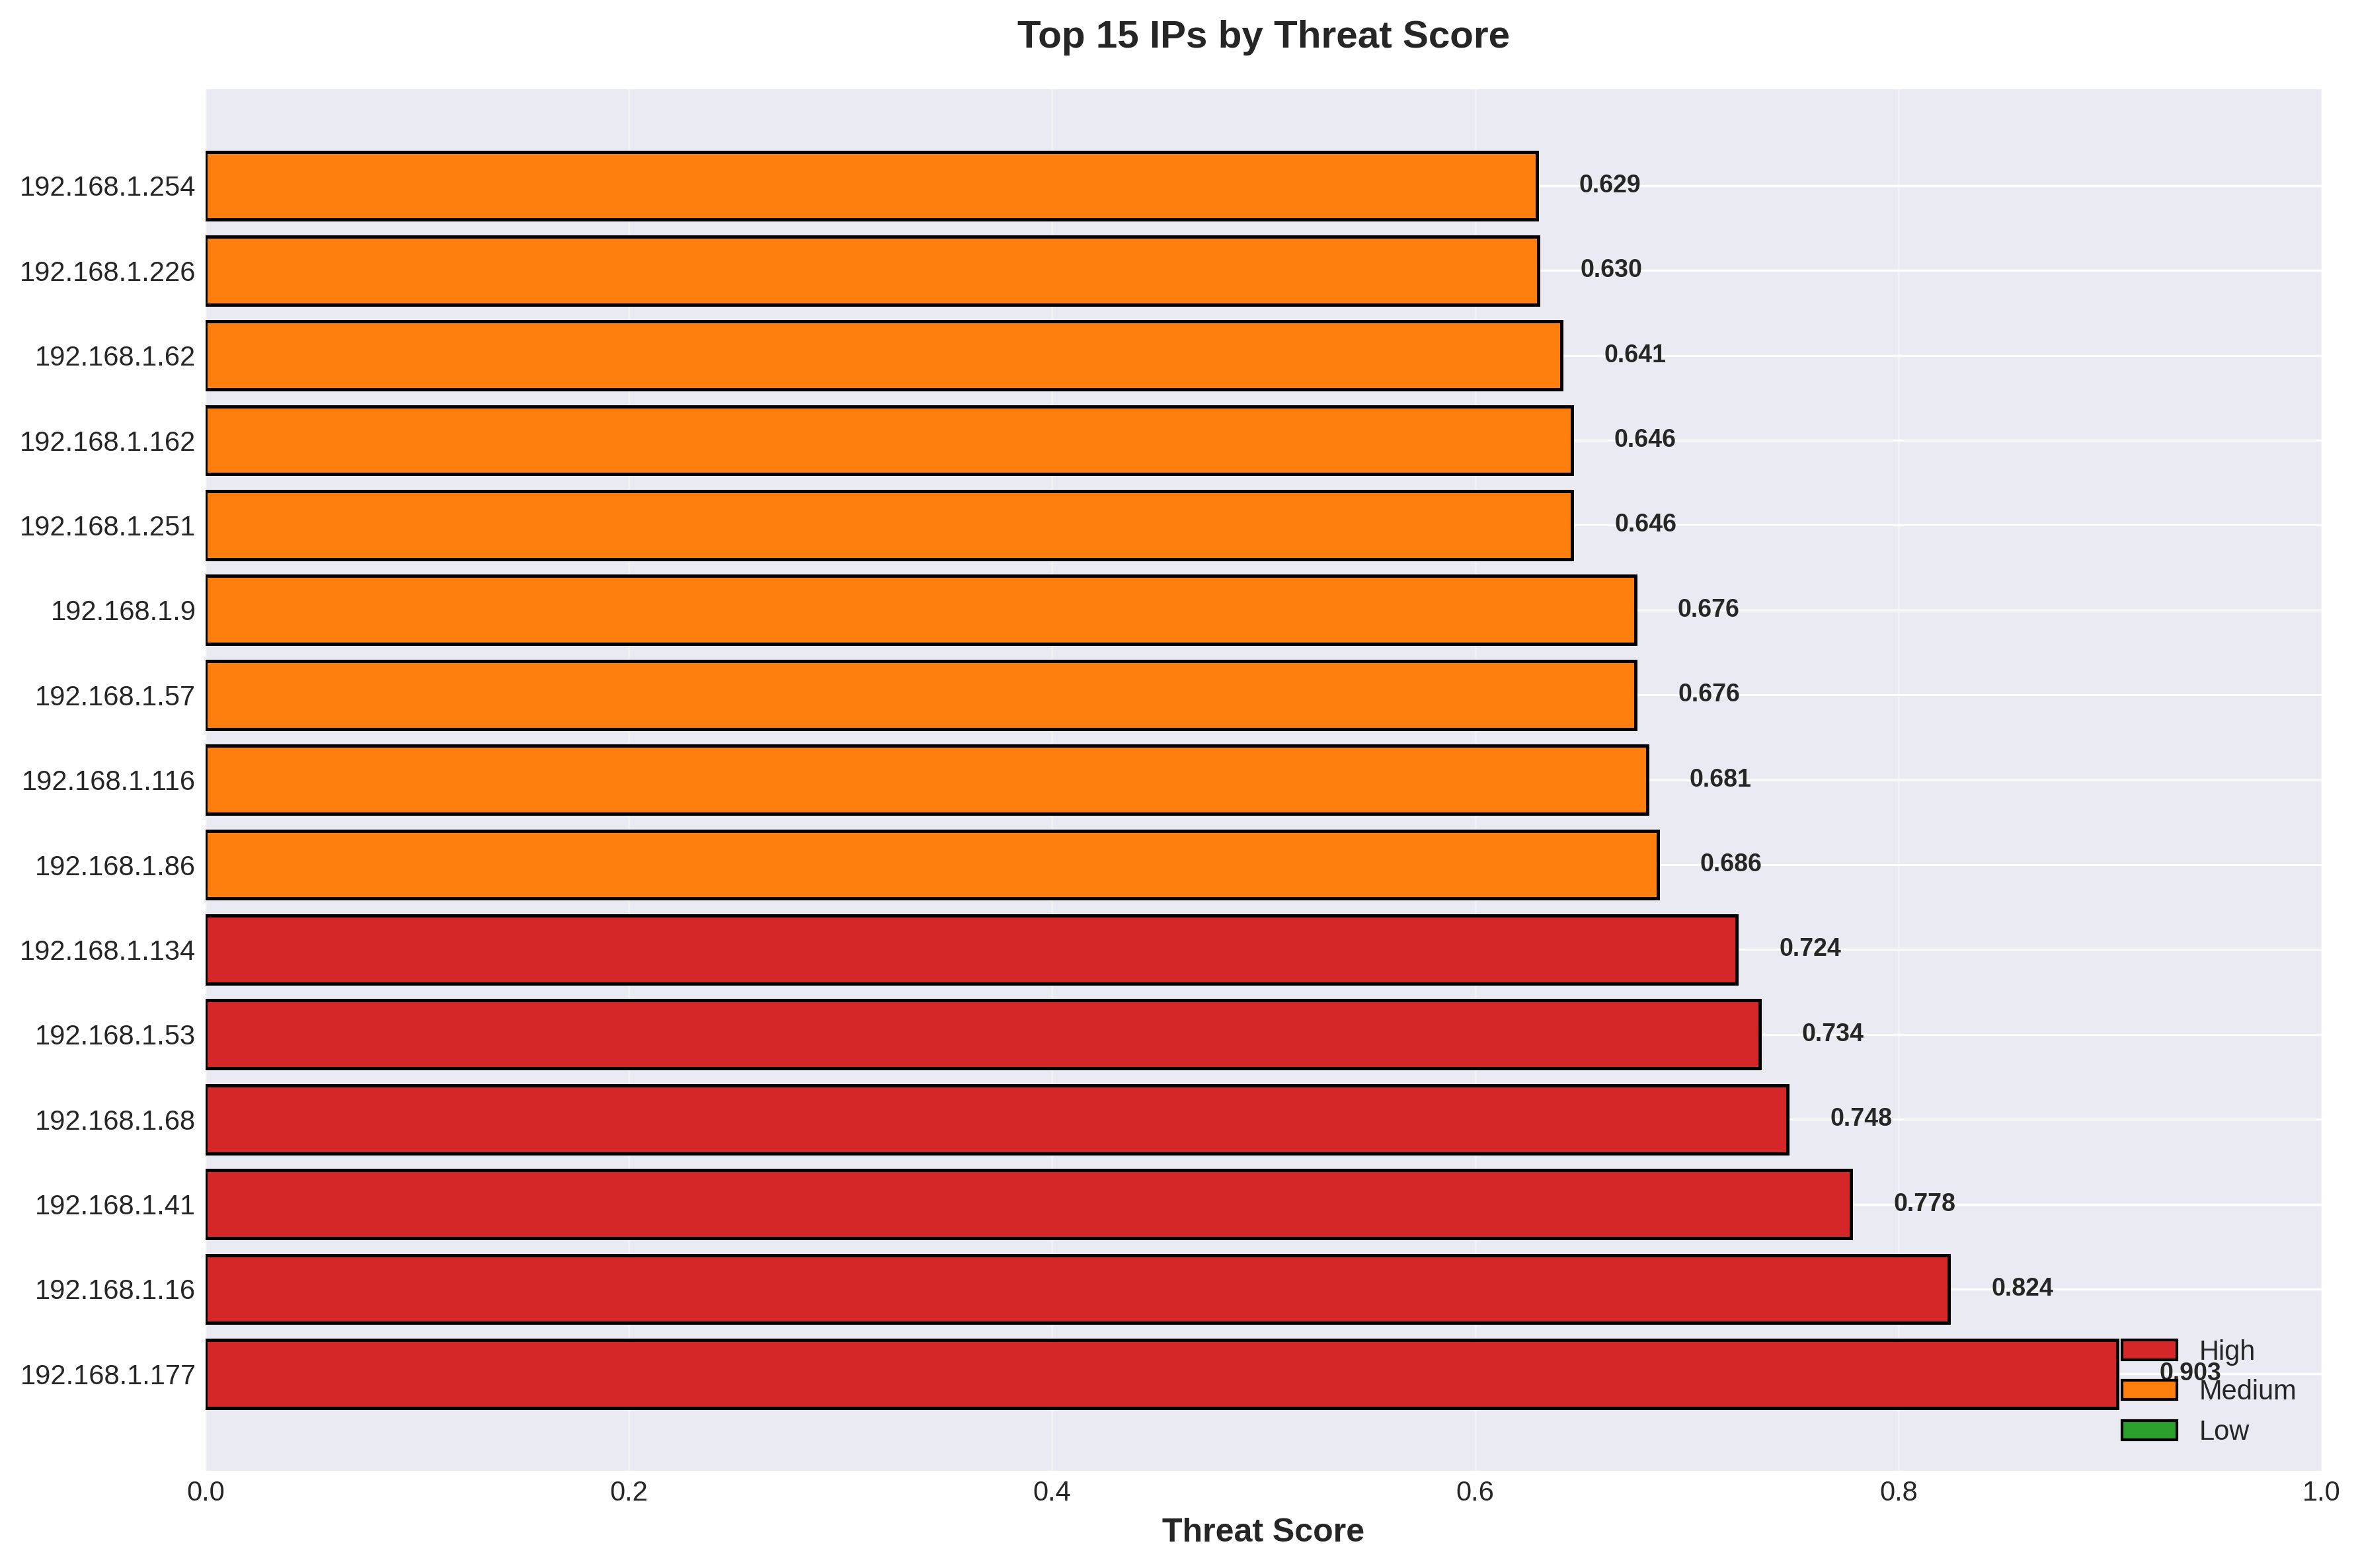
\includegraphics[width=0.95\textwidth]{plots/03_top_threat_ips.png}
\caption{Top 15 IPs ranked by threat score. Each IP is color-coded according to its threat level (High, Medium, Low). Higher threat scores indicate more suspicious behavior patterns.}
\label{fig:top_threat_ips}
\end{figure}

Key findings:
\begin{itemize}
    \item [INSERT TOP THREAT IPS ANALYSIS]
    \item High-risk IPs require immediate investigation
    \item Consider implementing firewall rules for top-ranked IPs
\end{itemize}

\subsection{Threat Level Distribution}

\begin{figure}[H]
\centering
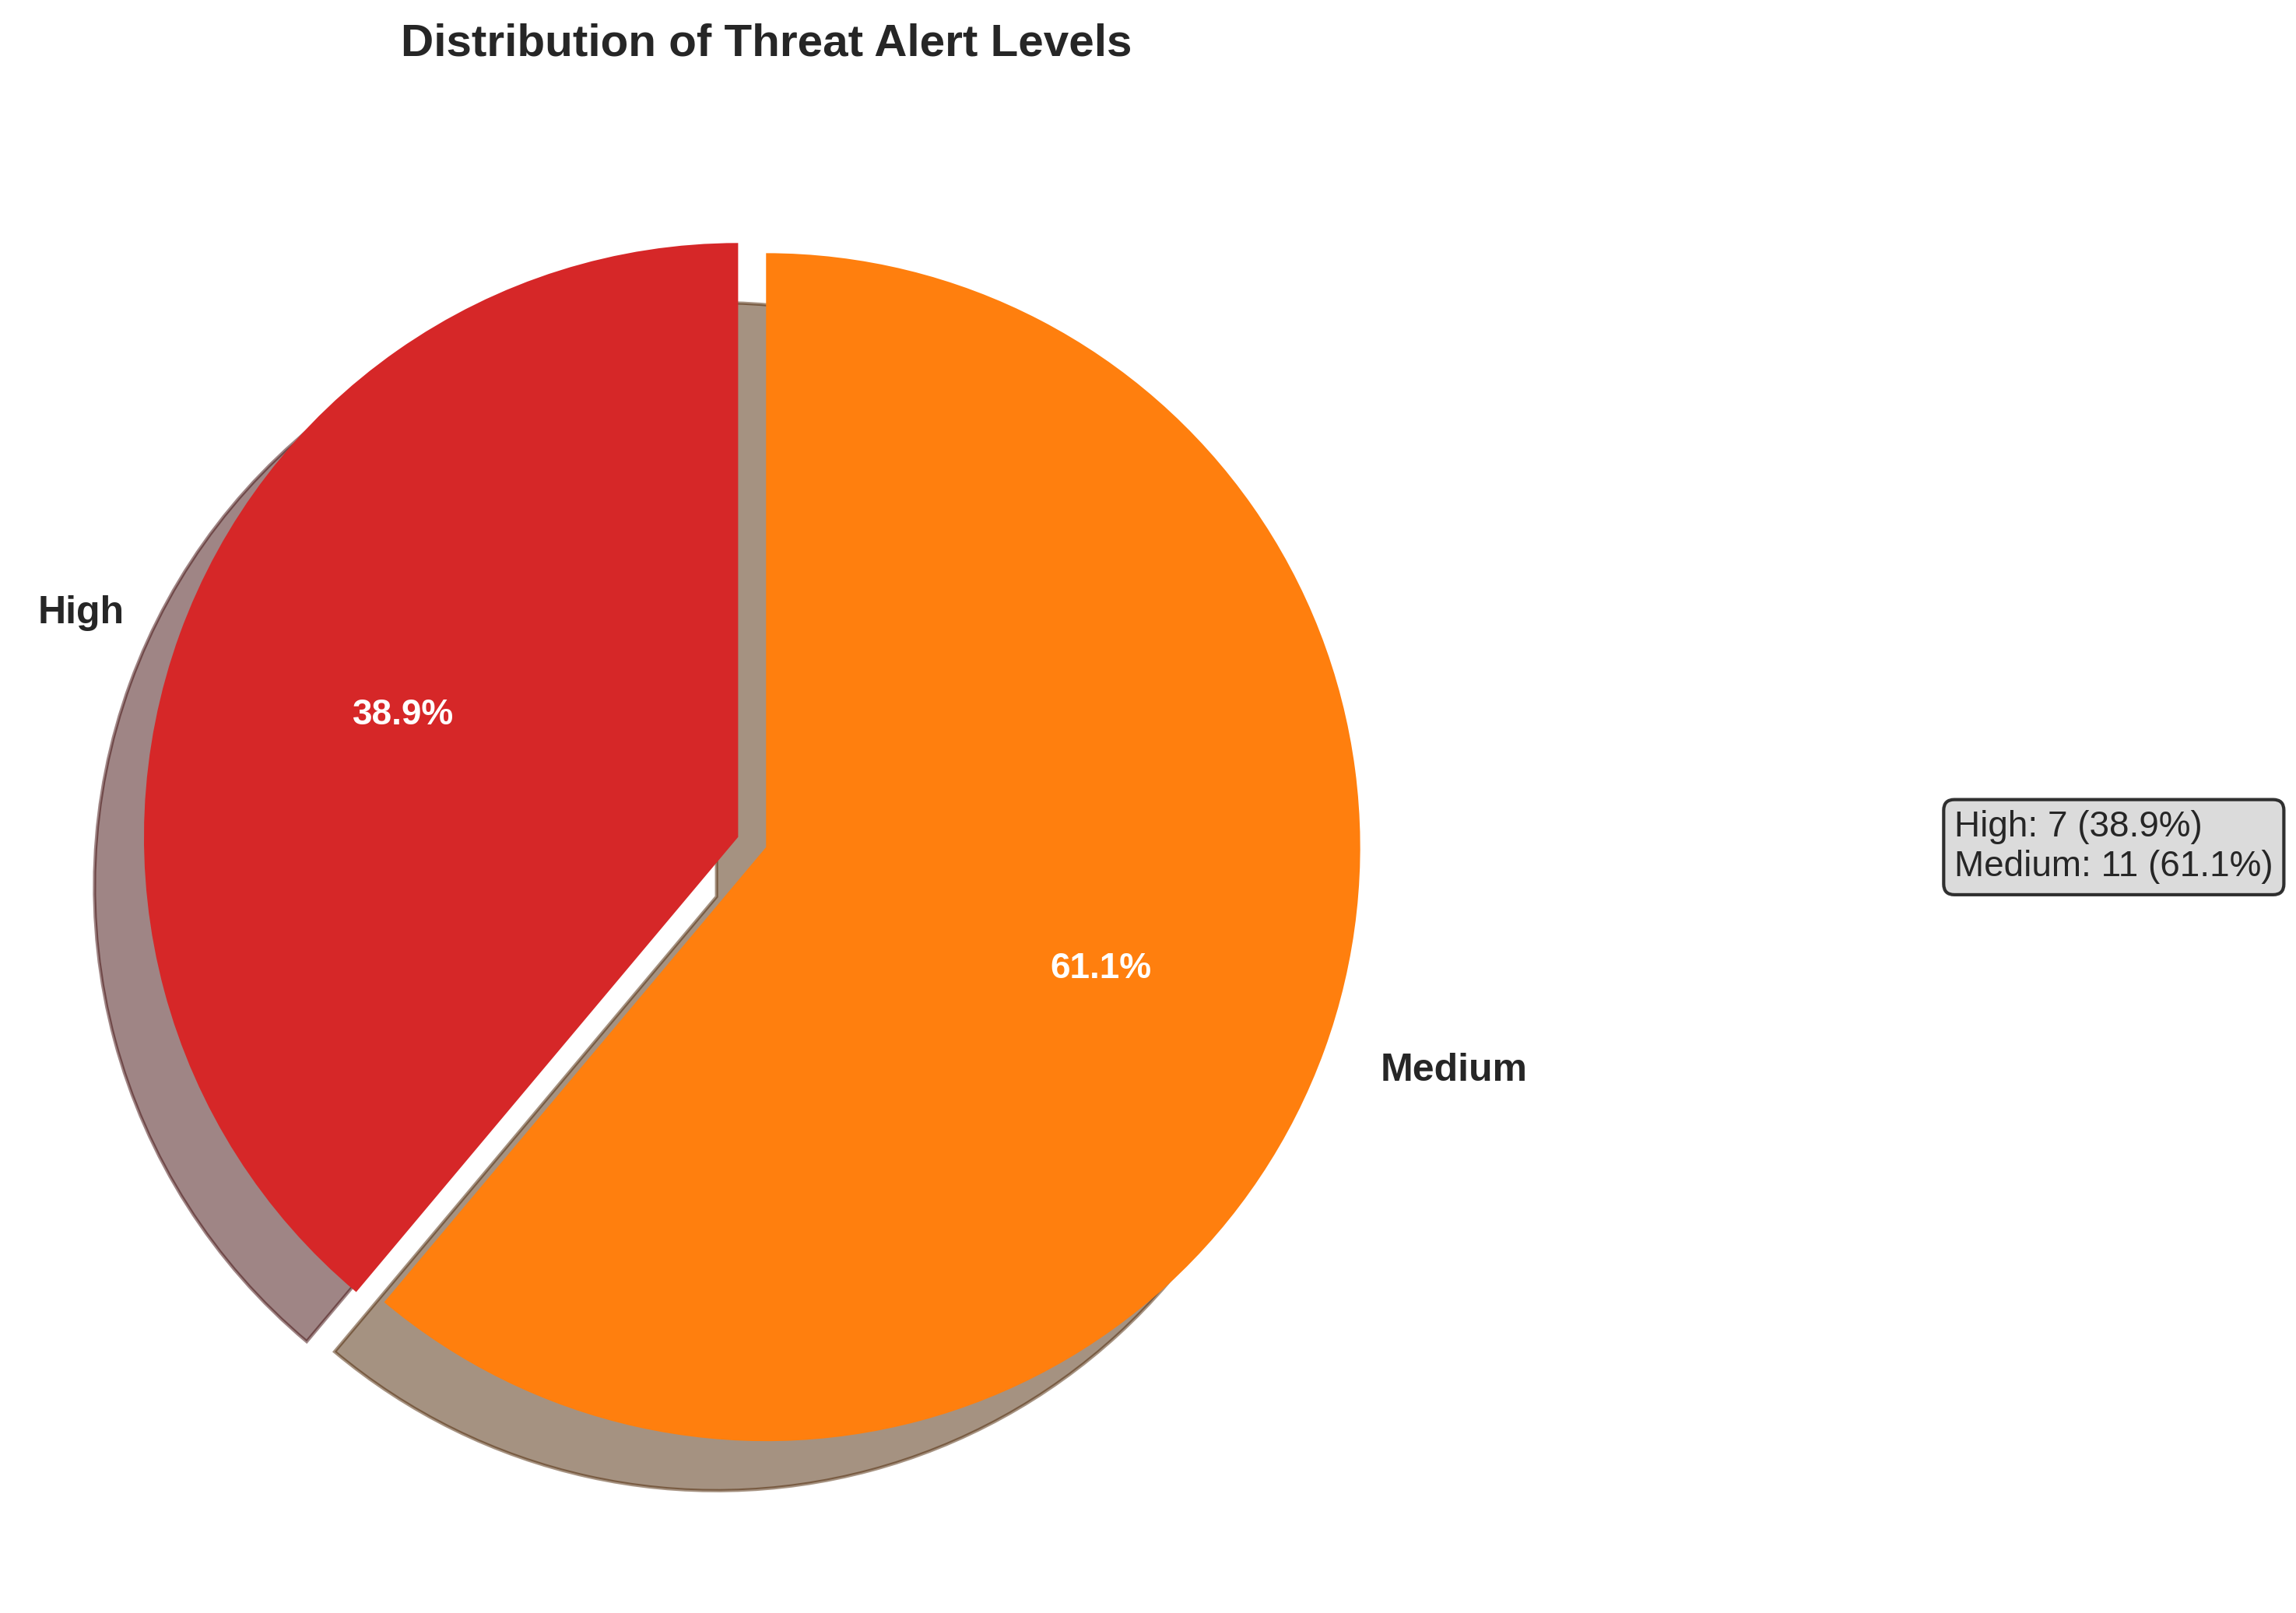
\includegraphics[width=0.8\textwidth]{plots/04_threat_level_distribution.png}
\caption{Pie chart showing the distribution of threat alerts across different threat levels. The distribution indicates the severity and frequency of detected threats.}
\label{fig:threat_dist}
\end{figure}

\section{Temporal Analysis}

\subsection{Traffic Volume Over Time}

\begin{figure}[H]
\centering
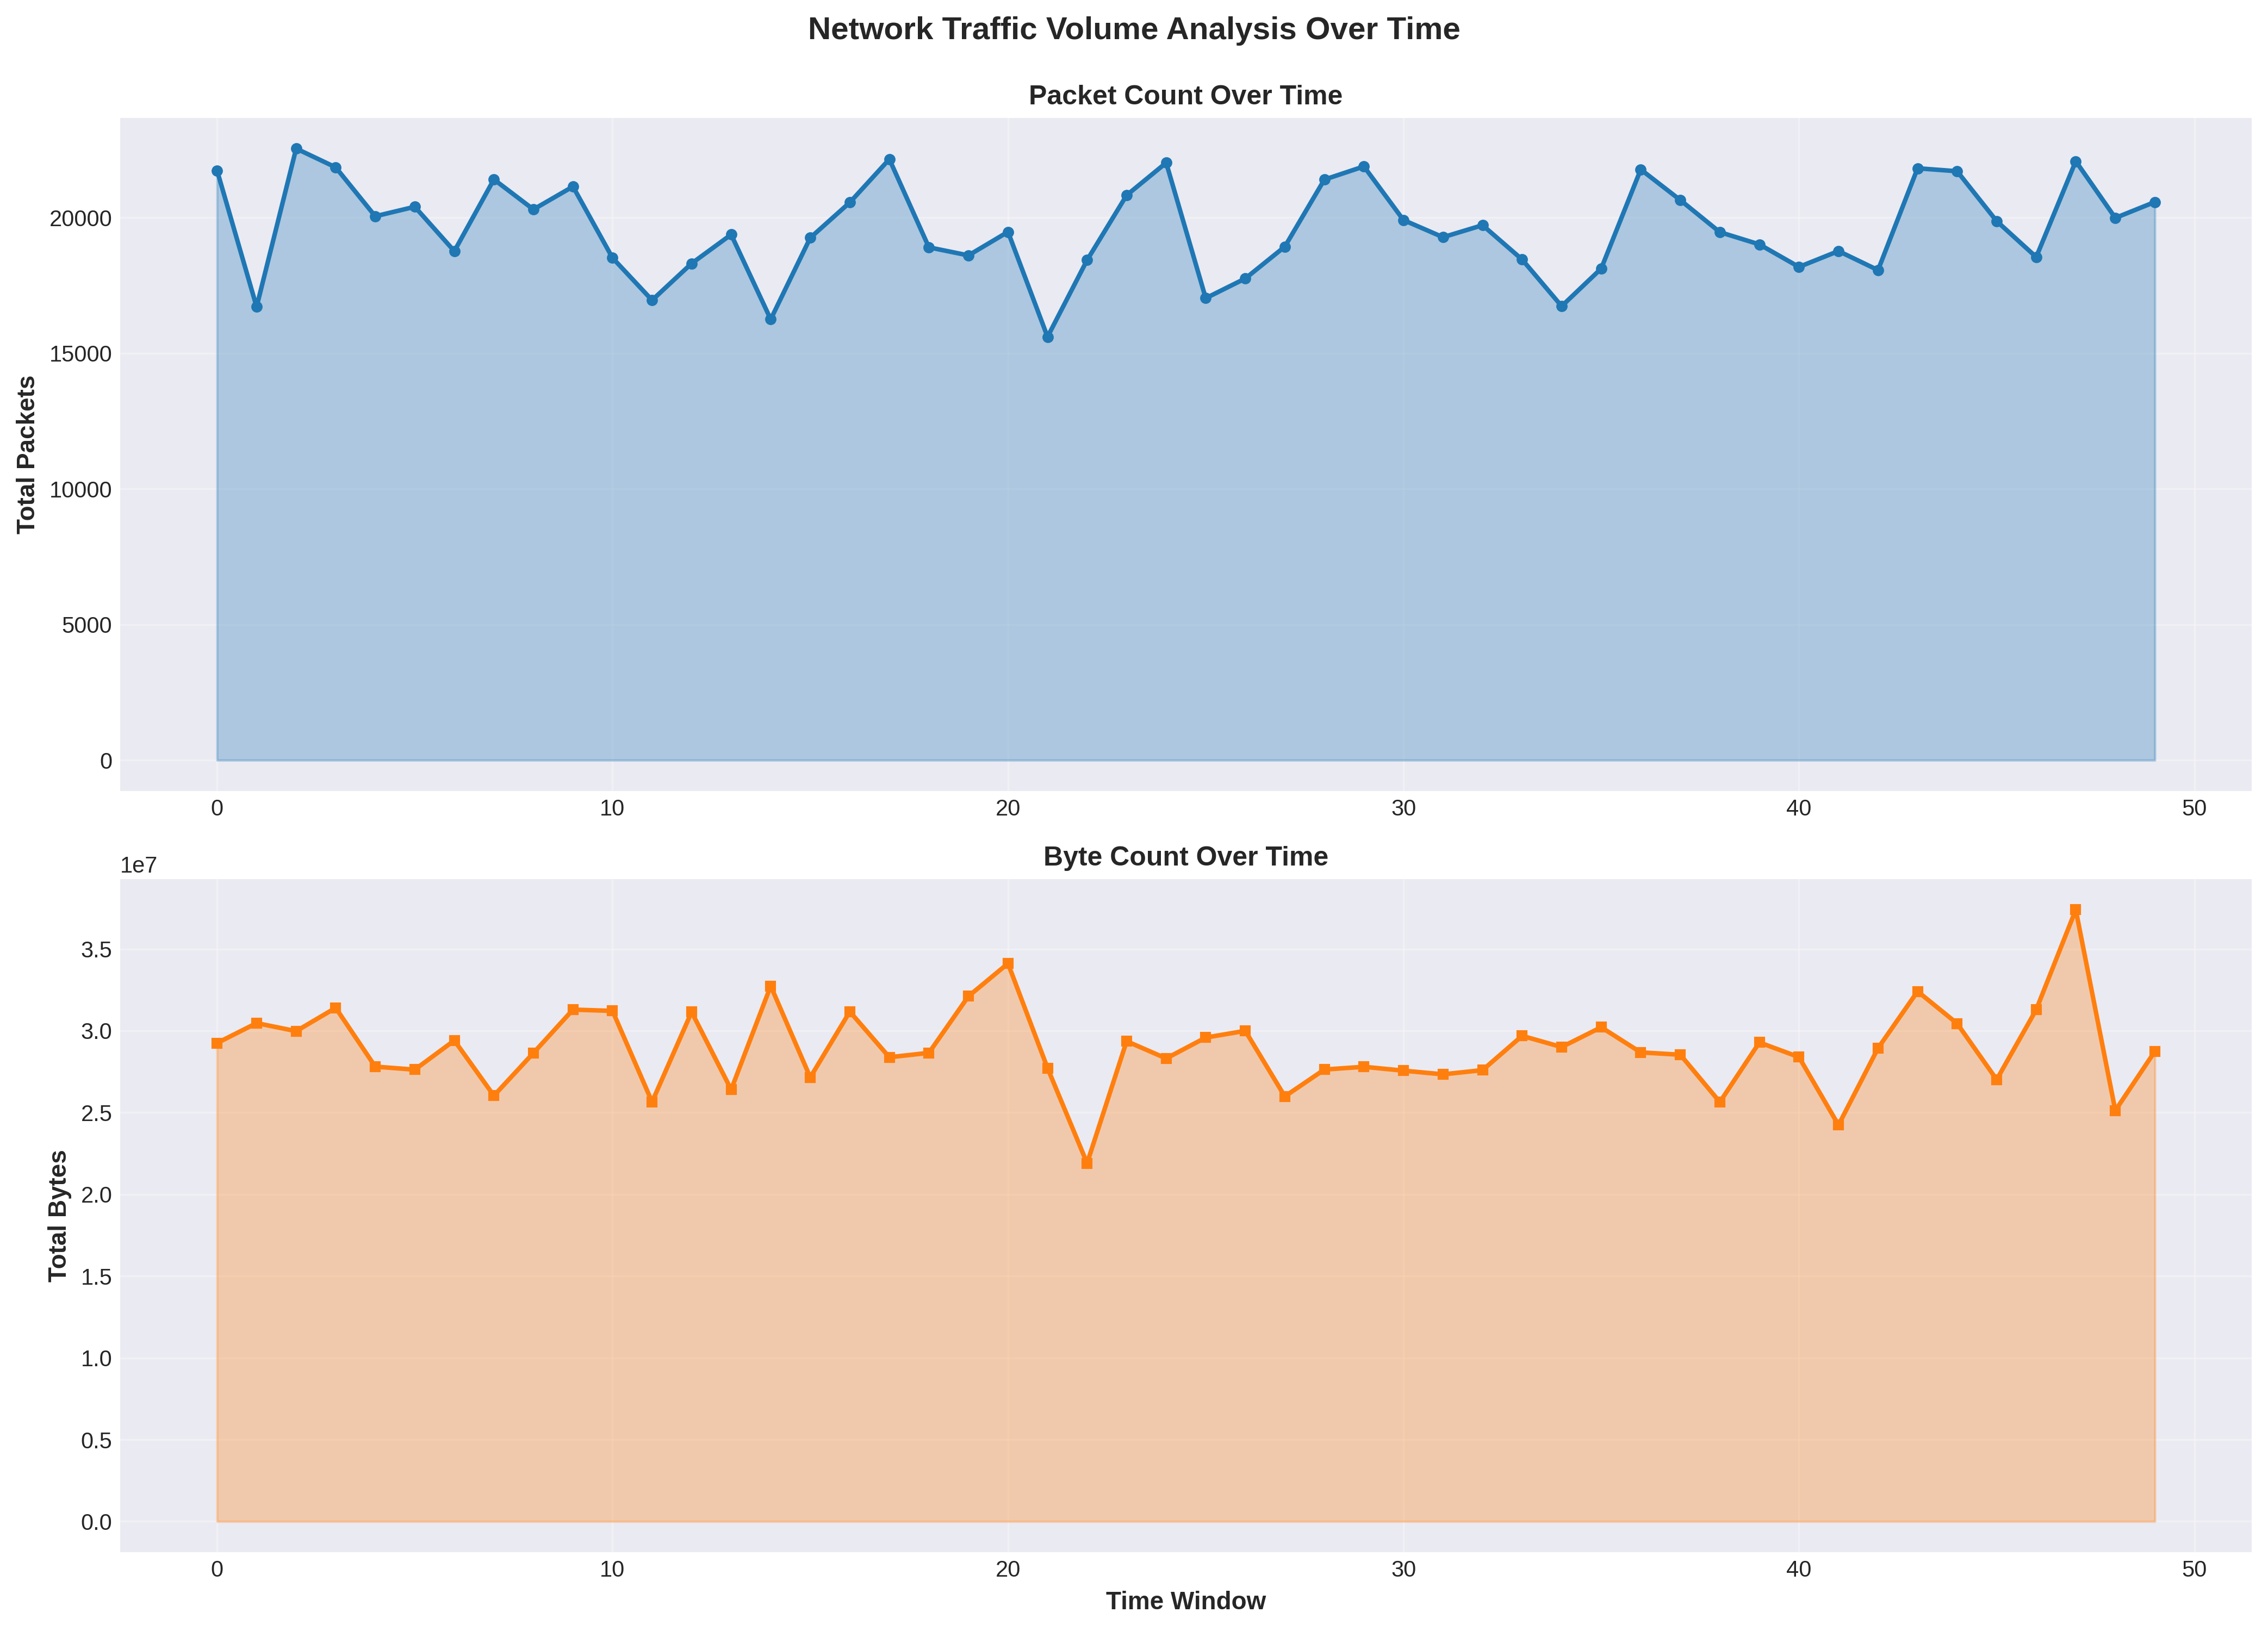
\includegraphics[width=0.95\textwidth]{plots/05_traffic_volume_over_time.png}
\caption{Temporal patterns of network traffic showing both packet count and byte count over time. This visualization helps identify traffic peaks, anomalies, and potential attacks at specific times.}
\label{fig:traffic_time}
\end{figure}

Observations:
\begin{itemize}
    \item [INSERT TEMPORAL PATTERN OBSERVATIONS]
    \item Time-based anomalies may correlate with specific attack behaviors
    \item Peak traffic periods should be monitored carefully
\end{itemize}

\section{Anomaly Scoring}

\subsection{Anomaly Score Distribution}

\begin{figure}[H]
\centering
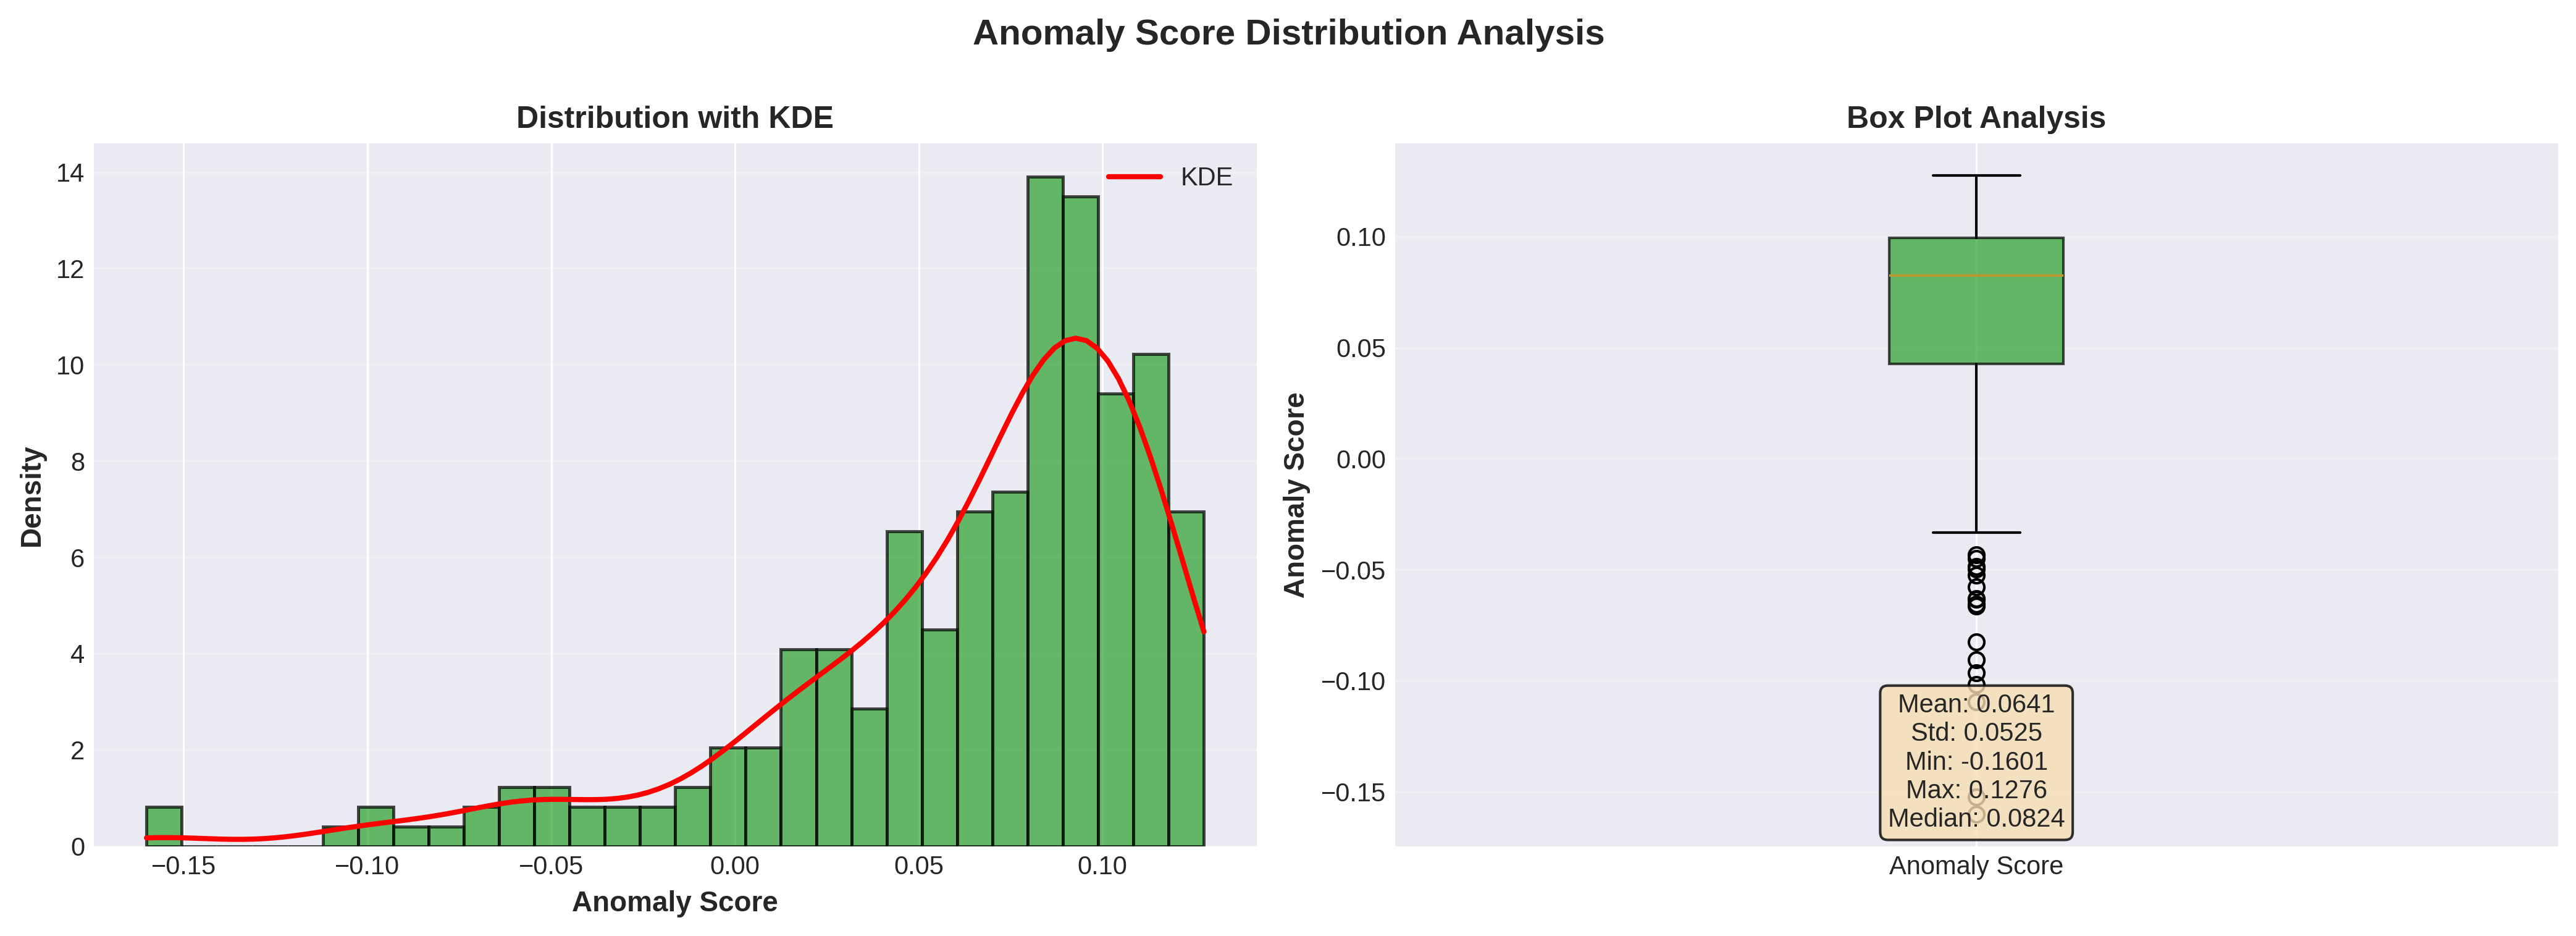
\includegraphics[width=0.95\textwidth]{plots/06_anomaly_score_distribution.png}
\caption{Distribution of anomaly scores computed for each IP. The left plot shows the histogram with kernel density estimation, while the right plot provides a box plot analysis with statistical summaries.}
\label{fig:anomaly_dist}
\end{figure}

Statistical insights:
\begin{itemize}
    \item Anomaly scores follow [INSERT DISTRIBUTION TYPE]
    \item Outliers indicate potentially malicious IPs
    \item The threshold for anomaly detection is based on statistical analysis
\end{itemize}

\section{Port Scanning Detection}

\subsection{Port Scanning Indicators}

\begin{figure}[H]
\centering
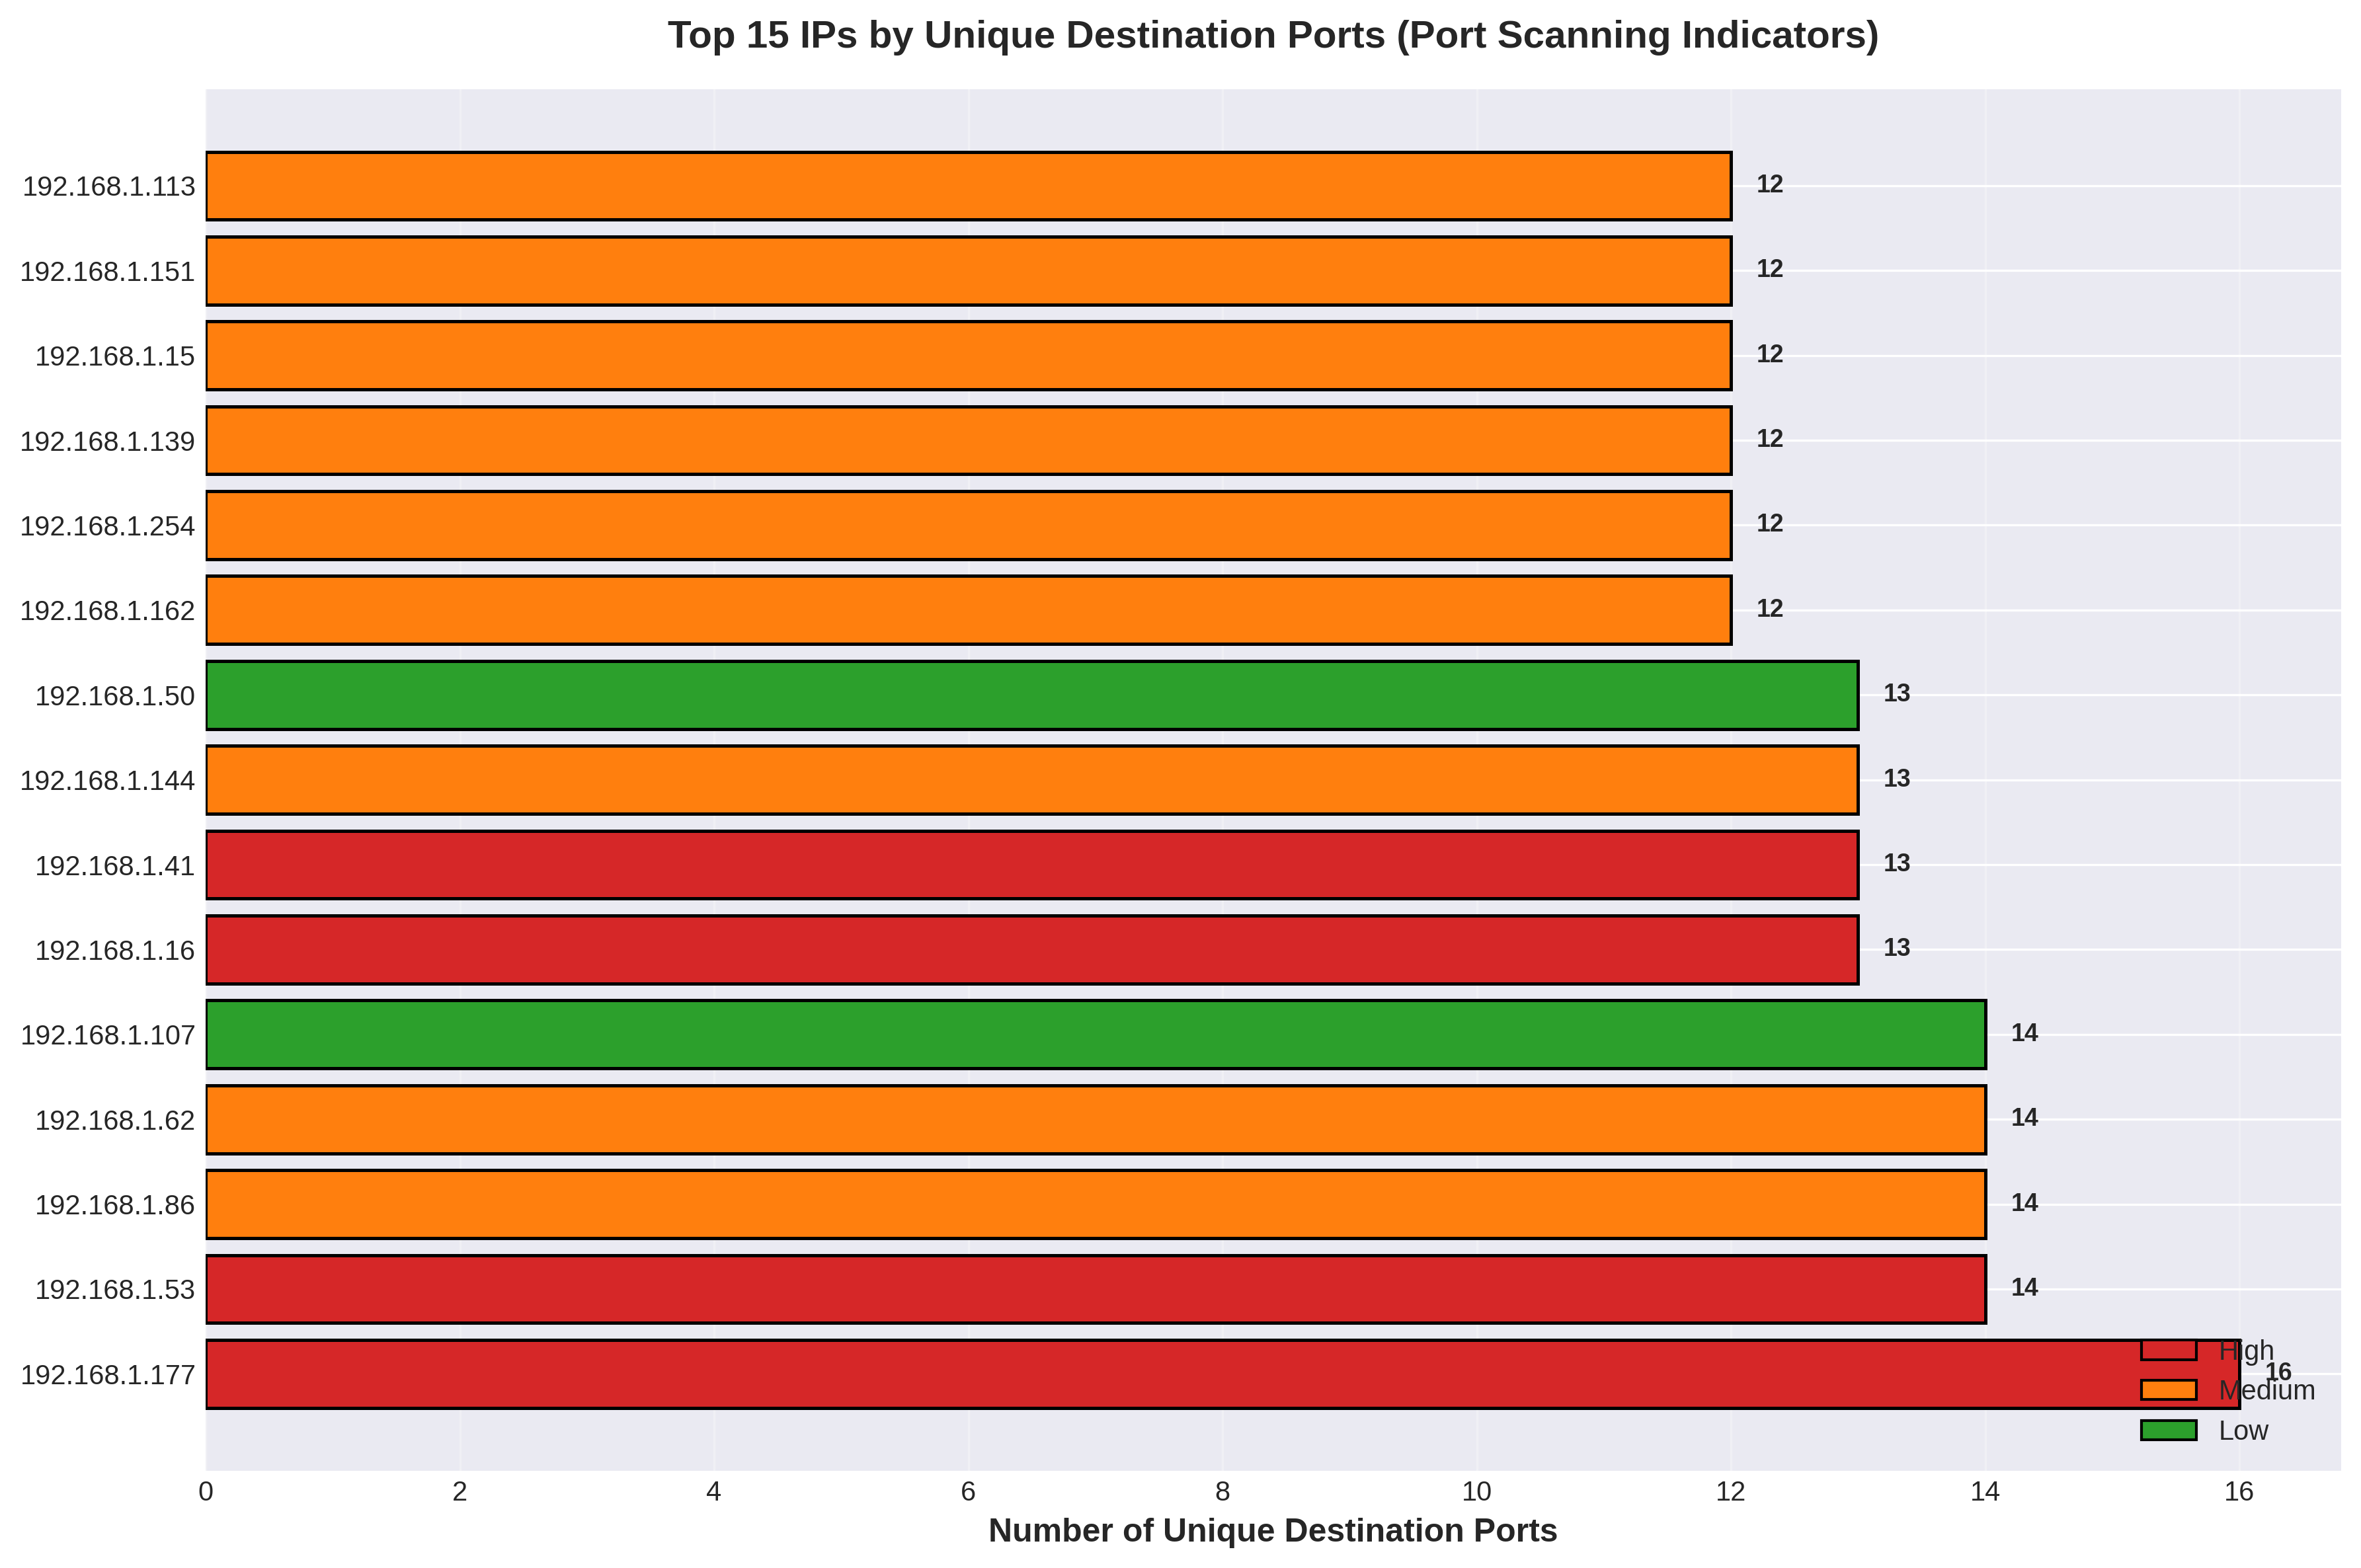
\includegraphics[width=0.95\textwidth]{plots/07_port_scanning_indicators.png}
\caption{Top 15 IPs by number of unique destination ports accessed. A high number of unique ports is a strong indicator of port scanning activity.}
\label{fig:port_scan}
\end{figure}

Port scanning analysis:
\begin{itemize}
    \item IPs scanning multiple ports are highly suspicious
    \item [INSERT PORT SCANNING OBSERVATIONS]
    \item These IPs should be prioritized for investigation
\end{itemize}

\section{Traffic Metrics Analysis}

\subsection{Packets vs Bytes Scatter Plot}

\begin{figure}[H]
\centering
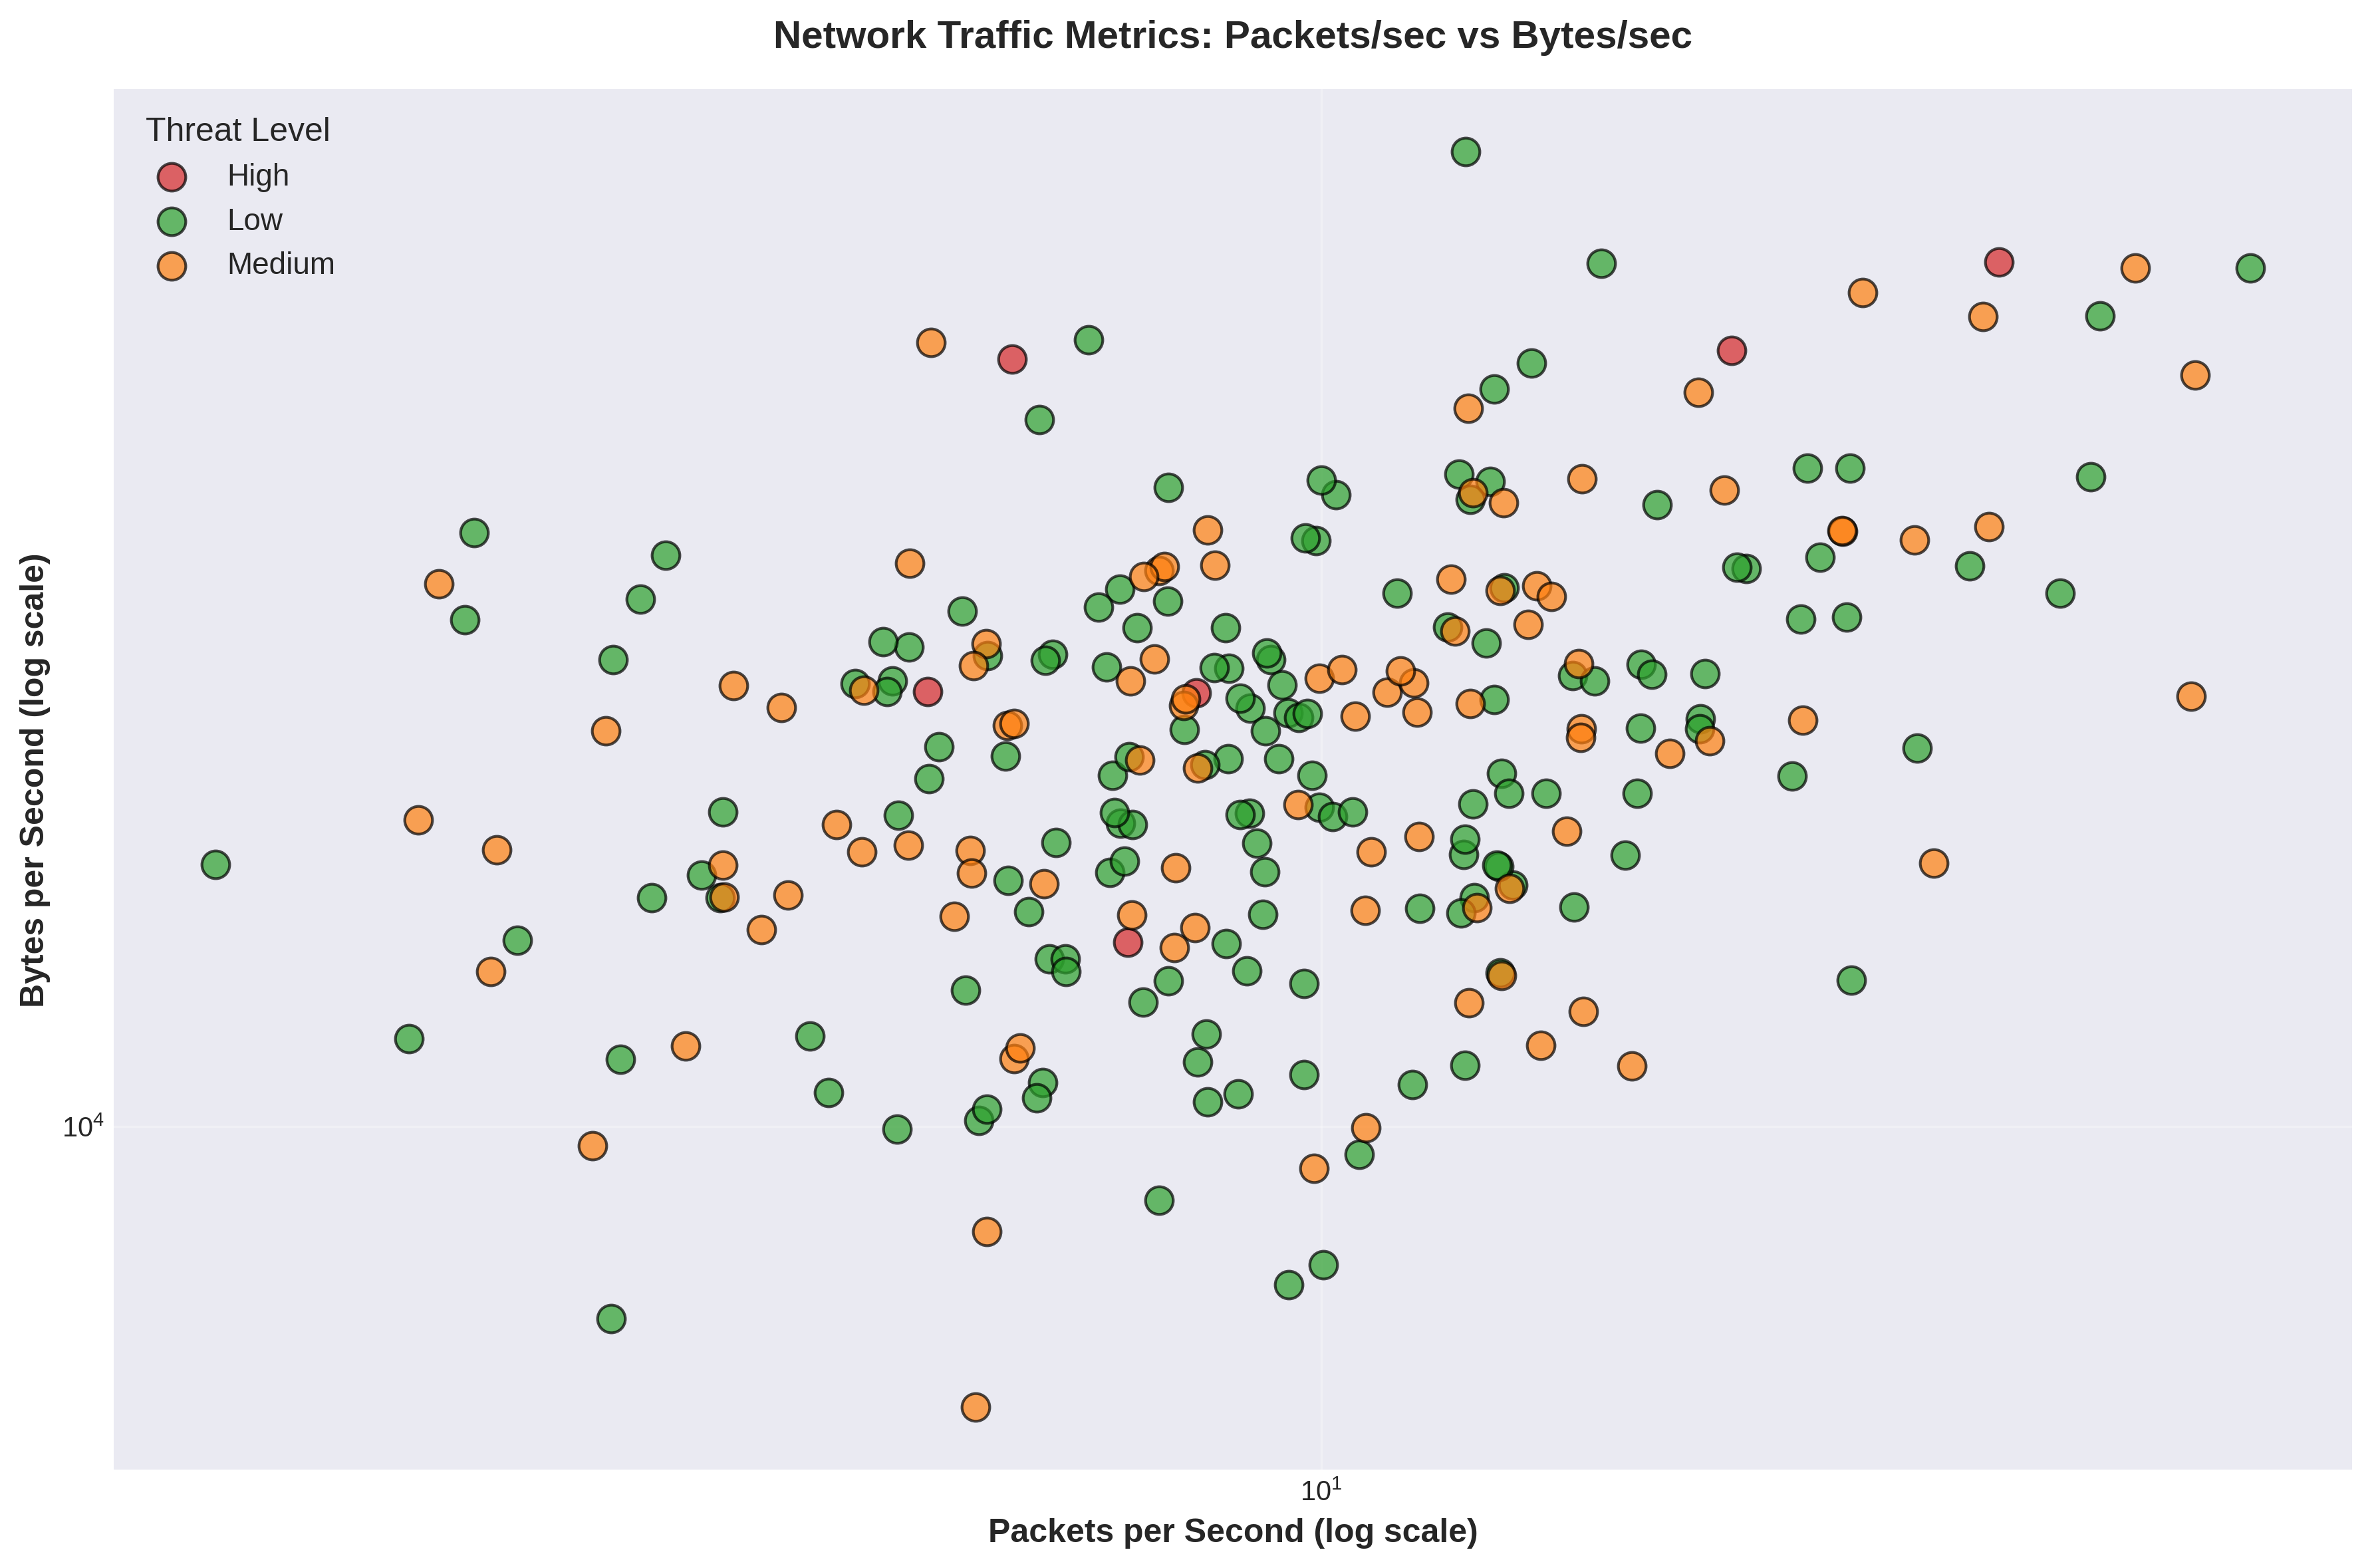
\includegraphics[width=0.95\textwidth]{plots/08_traffic_metrics_scatter.png}
\caption{Scatter plot comparing packets per second (x-axis) with bytes per second (y-axis), color-coded by threat level. Both axes use logarithmic scales to better visualize the full range of traffic patterns.}
\label{fig:scatter_metrics}
\end{figure}

Key patterns:
\begin{itemize}
    \item Different threat levels exhibit distinct traffic patterns
    \item High-threat IPs may show specific metric signatures
    \item [INSERT METRIC PATTERN OBSERVATIONS]
\end{itemize}

\section{Spike Detection}

\subsection{Anomalous Spikes Per Time Window}

\begin{figure}[H]
\centering
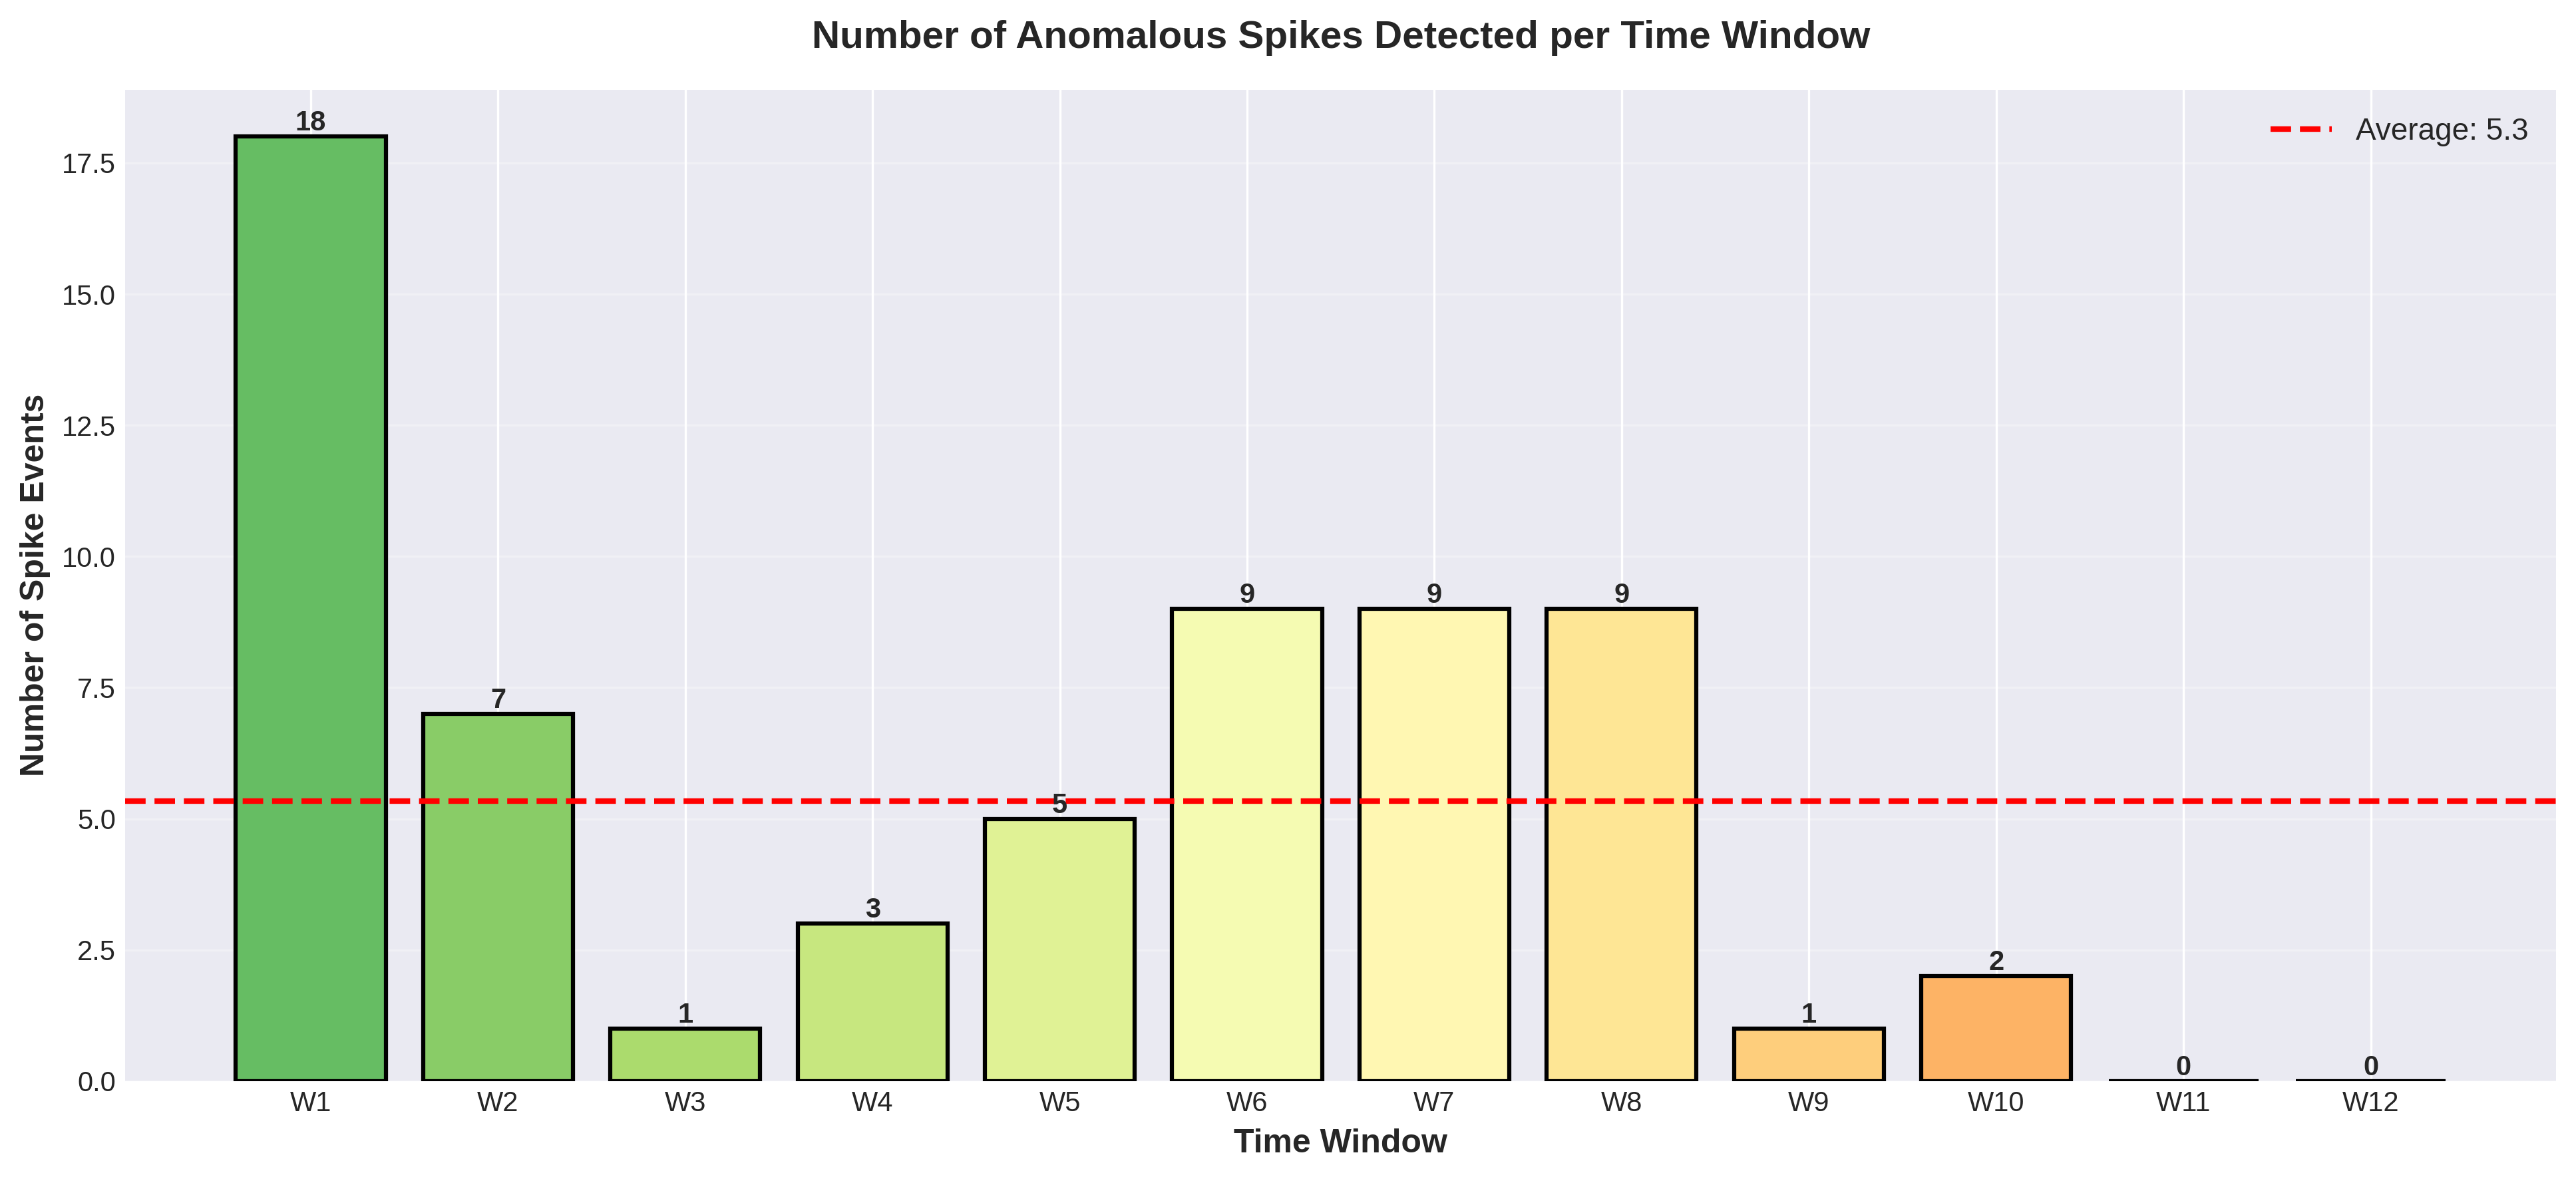
\includegraphics[width=0.95\textwidth]{plots/09_spike_detection_summary.png}
\caption{Number of detected anomalous spikes per time window. The red dashed line indicates the average number of spikes across all time windows.}
\label{fig:spike_detection}
\end{figure}

Spike analysis:
\begin{itemize}
    \item Time windows with elevated spike counts indicate periods of high anomaly
    \item Correlation with external events should be investigated
    \item [INSERT SPIKE PATTERN OBSERVATIONS]
\end{itemize}

% ============================================================================
% CHAPTER 4: CONCLUSIONS AND RECOMMENDATIONS
% ============================================================================
\chapter{Conclusions and Recommendations}

\section{Key Findings}

\begin{itemize}
    \item \textbf{Finding 1}: [INSERT KEY FINDING]
    \item \textbf{Finding 2}: [INSERT KEY FINDING]
    \item \textbf{Finding 3}: [INSERT KEY FINDING]
    \item \textbf{Finding 4}: [INSERT KEY FINDING]
\end{itemize}

\section{Security Recommendations}

\subsection{Immediate Actions}

\begin{enumerate}
    \item Investigate high-threat IPs identified in the analysis
    \item Implement firewall rules to block or monitor suspicious IPs
    \item Increase monitoring during peak traffic periods
    \item Review port scanning attempts and consider network segmentation
\end{enumerate}

\subsection{Medium-Term Improvements}

\begin{itemize}
    \item Integrate real-time alerts with SIEM systems
    \item Implement machine learning models for automated threat response
    \item Set up threat intelligence feeds for enhanced detection
    \item Conduct penetration testing based on identified vulnerabilities
\end{itemize}

\subsection{Long-Term Strategy}

\begin{itemize}
    \item Establish baseline behavior profiles for network IPs
    \item Implement behavioral analysis for early threat detection
    \item Develop incident response playbooks for identified threat types
    \item Continuously update detection algorithms with new threat intelligence
\end{itemize}

\section{Future Work}

\begin{itemize}
    \item Extend analysis to encrypted traffic patterns
    \item Integrate with external threat intelligence feeds
    \item Develop predictive models for threat forecasting
    \item Implement automated response mechanisms
\end{itemize}

\section{Conclusion}

The DINDGA system successfully identifies and analyzes network intrusions using advanced graph analysis and machine learning techniques. The generated visualizations and statistical analyses provide valuable insights for network security operations. Continued monitoring and refinement of detection algorithms are recommended to maintain security posture against evolving threats.

% ============================================================================
% APPENDICES
% ============================================================================
\appendix

\chapter{Technical Details}

\section{Environment and Dependencies}

The analysis was conducted using:
\begin{itemize}
    \item Python 3.9+
    \item Key libraries: pandas, numpy, scikit-learn, networkx, matplotlib, seaborn
    \item Analysis framework: DINDGA
\end{itemize}

\section{Data Processing Pipeline}

\begin{lstlisting}[language=Python, caption=Basic Data Loading Example]
import pandas as pd
import numpy as np

# Load network traffic data
network_data = pd.read_csv('network_traffic_data.csv')

# Load detection results
detection_results = pd.read_csv('detection_results.csv')

# Filter high-threat IPs
high_threat_ips = detection_results[
    detection_results['threat_score'] > 0.7
]

print(f"Found {len(high_threat_ips)} high-threat IPs")
\end{lstlisting}

\section{Plot Generation}

The visualization pipeline includes:
\begin{enumerate}
    \item Data extraction and preprocessing
    \item Statistical analysis and calculation
    \item Matplotlib/Seaborn rendering
    \item High-resolution PNG export (300 DPI)
\end{enumerate}

\chapter{References}

\begin{enumerate}
    \item [INSERT REFERENCE 1]
    \item [INSERT REFERENCE 2]
    \item [INSERT REFERENCE 3]
    \item Maloof, M., \& Stephens, G. (2007). ELICIT: A system for detecting insider threats from shell command logs.
    \item Chandola, V., Banerjee, A., \& Kumar, V. (2009). Anomaly detection: A survey. ACM Computing Surveys, 41(3), 1-58.
\end{enumerate}

\end{document}
